\documentclass[a4paper,11pt]{report}
\usepackage[T1]{fontenc}
\usepackage[utf8]{inputenc}
\usepackage{lmodern}
\usepackage{graphicx}

\title{\textbf{Sprawozdanie z laboratorium\\Stos i Kolejka}}
\author{Adam Dąbrowski 184208}
\begin{document}
\maketitle
\section{Wprowadzenie}

Celem ćwiczenia było zapoznanie się z klasmi pojemnikowymi - stosem i kolejką. Stos jest to pojemnik typu LIFO(last in first out) ostatni element jaki kładziemy na stos zdejmujemy z niego jako pierwszy. Kolejka jest to pojemnik typu FIFO(first in first out) wyjmujemy z niej elementy w takiej samej kolejności w jakiej wczytywaliśmy.  

\section{Realizacjia}

Oba te pojemniki napisałem w oparciu o tablicę dynamiczną. Ważną kwestią jest tutaj zarządzanie pamięcią tak, żeby bez potrzeby jej nie marnować. 
Zarówno w stosie jak i w kolejce przetestowałem dwa sobosoby alokowania pamięci: dwukrotne powiększanie rozmiaru tablicy i mozolne rozszerzanie o jeden element. W przypadku kolejki zanim zwiększę jej rozmiar sprawdzam czy mogę przesunąć wszystkie elementy do przodu, robiąc w ten sposób miejsce na kolejne. W obu przypadkach pojemniki zmniejszam o połowę wtedy kiedy dane wypełniają pojemnik w jednej czwartej. Program sprawdzam wkładając, a następnie wyjmując kolejno 1, 10, 100 ,1000,10 000, 100 000 liczb typu całkowitego. Operacje te przeprowadzam 300 razy, przy tej liczbie przy prawie każdym uruchomieniu dostaję podobne wyniki, a następnie liczę z tego średni czas. 
\newpage
\section{STOS}
\begin{tabular}{|rl|}
\hline
\multicolumn{2}{|c|}{powiększanie o jeden}\\
\hline
ilosc elementow & czas - nano sekundy\\
\hline
1&437\\
10&3809\\
100&62617\\
1000&2330166\\
10000&11008400\\
\hline
\end{tabular}

\begin{figure}
  \begin{center}
    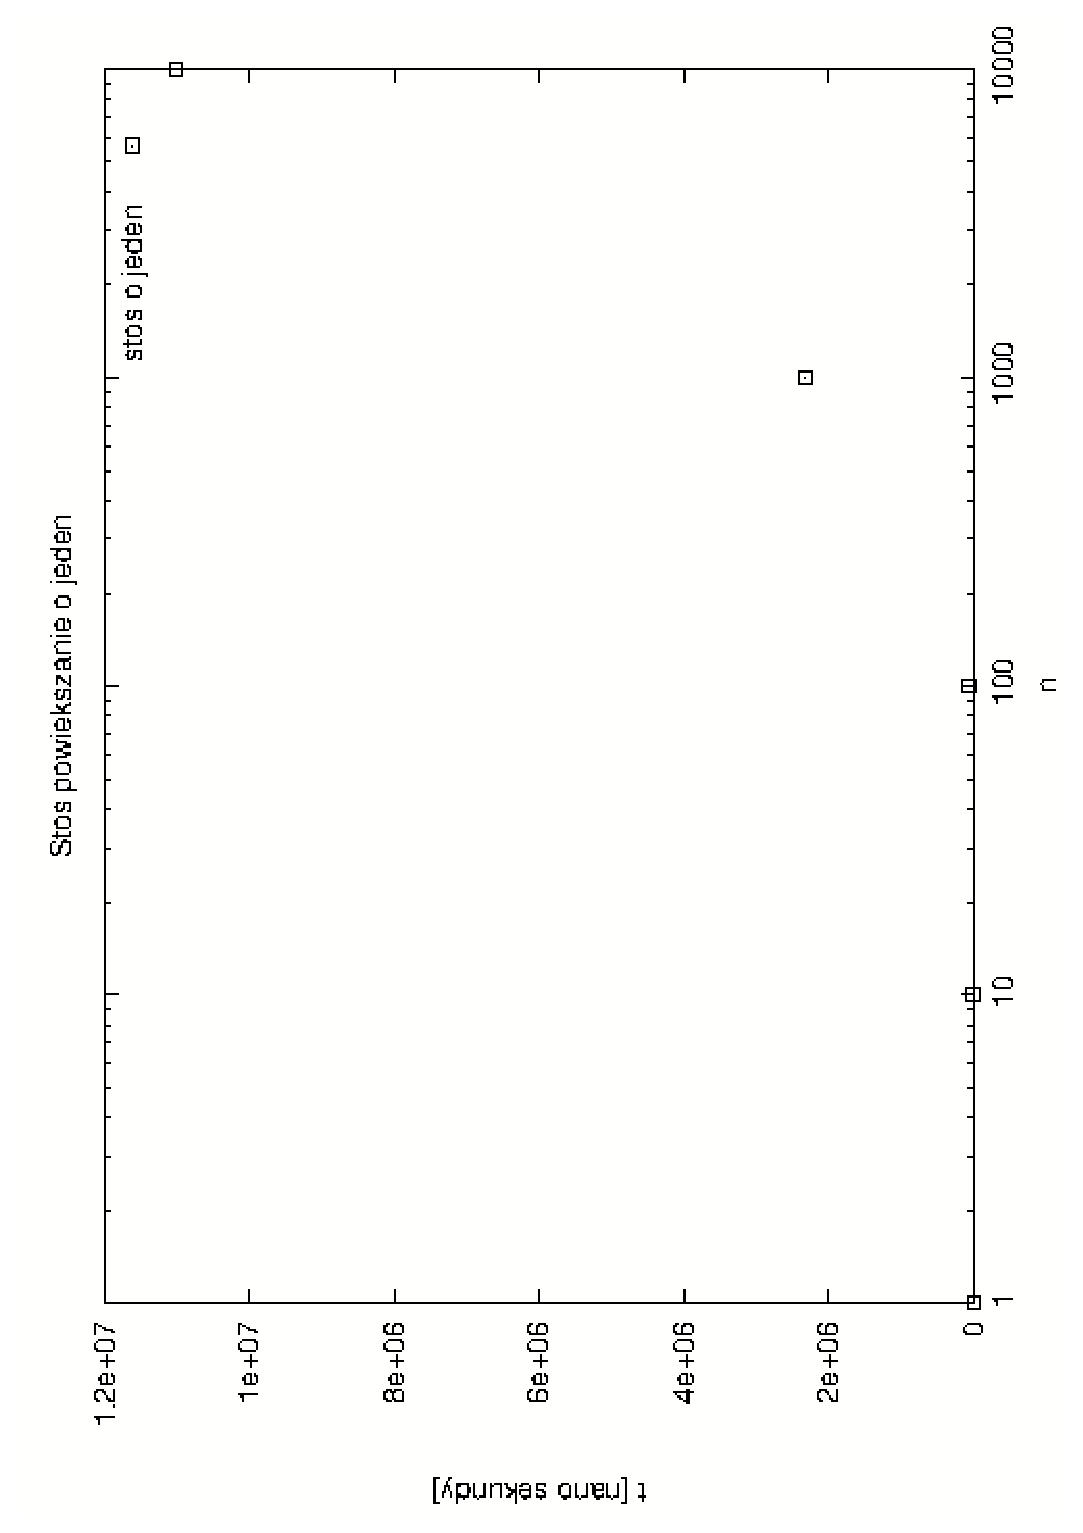
\includegraphics{wykresy/stos_o_jeden.eps}
    \caption{}
    \label{fig:}
  \end{center}
\end{figure}
\begin{tabular}{|rl|}
\hline
\multicolumn{2}{|c|}{powiększanie dwa razy}\\
\hline
ilosc elementow & czas - nano sekundy\\
\hline
1&445\\
10&2366\\
100&14249\\
1000&26683\\
10000&272685\\
100000&2648233\\
\hline
\end{tabular}

\begin{figure}
  \begin{center}
    \includegraphics{wykresy/stos_x_dwa.eps}
    \caption{}
    \label{fig:}
  \end{center}
\end{figure}

\section{KOLEJKA}
\begin{tabular}{|rl|}
\hline
\multicolumn{2}{|c|}{powiększanie o jeden}\\
\hline
ilosc elementow & czas - nano sekundy\\
\hline
1&481\\
10&964\\
100&73007\\
1000&2341611\\
10000&1424870\\
\hline
\end{tabular}

\begin{figure}
  \begin{center}
    \includegraphics{wykresy/kolejka_o_jeden.eps}
    \caption{}
    \label{fig:}
  \end{center}
\end{figure}

\begin{tabular}{|rl|}
\hline
\multicolumn{2}{|c|}{powiększanie dwa razy}\\
\hline
ilosc elementow & czas - nano sekundy\\
\hline
1&119\\
10&669\\
100&4030\\
1000&32699\\
10000&294486\\
100000&2992501\\
\hline
\end{tabular}

\begin{figure}
  \begin{center}
    \includegraphics{wykresy/kolejka_x_dwa.eps}
    \caption{}
    \label{fig:}
  \end{center}
\end{figure}

\section{Wnioski}
Powiększanie tablicy o jeden w obu wypadkach jest najgorszym rozwiązaniem z możliwych. W wariancie z powiększaniem o jeden element musiałem zmniejszyć liczbę danych o rząd ponieważ komputer nie mógł ukończyć tego programu - po dwudziestu minutach na siłę wyłączyłem program.
Oba typy pojemników mają zbliżoną wydajność, jednak kolejka zdaje się działać szybciej. Jest to dla mnie dość dziwne ponieważ oba pojemniki są oparte o działającą w podobny sposób tablicę dynamiczną.

\end{document}
